\documentclass[12pt, a4paper]{article}

% --- Packages ---
\usepackage[utf8]{inputenc}
\usepackage[T1]{fontenc}
\usepackage{palatino}
\usepackage[margin=2.5cm]{geometry}
\usepackage{microtype}
\usepackage{setspace}
\usepackage{titlesec}
\usepackage{titling}
\usepackage{abstract}
\usepackage{booktabs}
\usepackage{array}
\usepackage{tabularx}
\usepackage{xcolor}
\usepackage{hyperref}

\usepackage{mdframed}
\usepackage{enumitem}
\usepackage{float}
\usepackage{caption}

% TikZ
\usepackage{tikz}
\usetikzlibrary{arrows.meta, positioning, decorations.pathreplacing, bending}

% --- Colors ---
\definecolor{uiblue}{RGB}{26,60,110}
\definecolor{ezpurple}{RGB}{74,46,122}
\definecolor{kernelbrown}{RGB}{122,58,26}
\definecolor{hwgreen}{RGB}{26,90,26}
\definecolor{digitalteal}{RGB}{26,90,74}
\definecolor{patchgold}{RGB}{90,74,26}
\definecolor{lightblue}{RGB}{240,245,252}
\definecolor{lightpurple}{RGB}{245,240,252}
\definecolor{lightorange}{RGB}{252,245,240}
\definecolor{lightgreen}{RGB}{240,248,240}
\definecolor{lightteal}{RGB}{240,252,250}
\definecolor{lightyellow}{RGB}{252,250,240}
\definecolor{rulecolor}{RGB}{180,180,180}
\definecolor{blockquotegray}{RGB}{100,100,100}

% --- Typography ---
\setstretch{1.35}
\setlength{\parskip}{6pt}
\setlength{\parindent}{0pt}

% Section formatting
\titleformat{\section}{\large\bfseries\color{uiblue}}{}{0em}{}[\vspace{2pt}\hrule\vspace{4pt}]
\titleformat{\subsection}{\normalsize\bfseries\color{ezpurple}}{}{0em}{}
\titleformat{\subsubsection}{\normalsize\itshape\color{kernelbrown}}{}{0em}{}

\titlespacing{\section}{0pt}{18pt}{8pt}
\titlespacing{\subsection}{0pt}{12pt}{4pt}

% Blockquote environment
\newmdenv[%
  leftline=true, rightline=false, topline=false, bottomline=false,
  linewidth=3pt, linecolor=rulecolor,
  innerleftmargin=12pt, innerrightmargin=0pt,
  innertopmargin=4pt, innerbottommargin=4pt,
  backgroundcolor=white,
  fontcolor=blockquotegray,
  font=\itshape\small
]{bquote}

% Hyperref setup
\hypersetup{
  colorlinks=true,
  linkcolor=uiblue,
  citecolor=kernelbrown,
  urlcolor=digitalteal
}

% --- Title ---
\title{%
  {\Large\bfseries The Anatomy of Sanctuaries}\\[6pt]
  {\normalsize The Dual Structure of the Modern State OS\\
  and the Mediterranean Deep Kernel}\\[4pt]
  {\small\itshape --- A 500-Year Architecture of Power
  Structurally Revealed by the Epstein Affair ---}
}
\author{Yuji Marutani}
\date{Version 1.1}

% ============================================================
\begin{document}
% ============================================================

% ============================================================
% COVER PAGE
% ============================================================
\begin{titlepage}
\newgeometry{top=2.8cm, bottom=2.8cm, left=3cm, right=3cm}
\thispagestyle{empty}

% Top rule
\noindent\rule{\textwidth}{1.2pt}\\[-4pt]
\noindent\rule{\textwidth}{0.3pt}

\vspace{2.6cm}

% Main title block
\begin{flushleft}
  {\fontsize{28}{34}\selectfont\bfseries The Anatomy of Sanctuaries}\\[14pt]
  {\fontsize{15}{20}\selectfont\mdseries
    The Dual Structure of the Modern State OS\\[4pt]
    and the Mediterranean Deep Kernel}\\[18pt]
  {\fontsize{11}{15}\selectfont\itshape\color{blockquotegray}
    --- A 500-Year Architecture of Power\\[2pt]
    \hspace{2em}Structurally Revealed by the Epstein Affair ---}
\end{flushleft}

\vspace{1.8cm}
\noindent\rule{\textwidth}{0.3pt}
\vspace{1.2cm}

% Abstract
\begin{flushleft}
  {\small\bfseries Abstract}\\[6pt]
  {\small\setstretch{1.4}%
  This paper presents a structural model for understanding how power operates
  through layered governance architectures. It argues that the institutions of
  modern democracy, rule of law, and territorial sovereignty constitute a
  visible \emph{user interface} (UI) of governance, beneath which persists a
  deeper network logic --- here termed the \emph{Mediterranean deep kernel} ---
  composed of transnational commercial, financial, and kinship structures
  predating the modern state. Drawing on Braudel's \emph{longue dur\'ee},
  Schmitt's theory of exception, and Arrighi's analysis of hegemonic cycles,
  the paper traces recurring structural logics from military-religious orders
  and chartered companies to contemporary offshore finance and digital
  sovereignty. The Epstein affair is examined not as proof of this model but
  as a \emph{moment of structural visibility}: an instance in which ordinarily
  opaque network power became publicly legible. The paper concludes by
  examining artificial intelligence as an emergent exception zone, and
  transparency events as periodic OS-level interventions by the state.
  }
\end{flushleft}

\vspace{1cm}
\noindent\rule{\textwidth}{0.3pt}
\vspace{1cm}

% Author / metadata block
\begin{flushleft}
  \begin{tabular}{@{}ll}
    {\small\bfseries Author} & {\small Yuji Marutani}\\[4pt]
    {\small\bfseries Version}                 & {\small 1.1}\\[4pt]
    {\small\bfseries Classification}          & {\small Working Paper --- Theoretical Model}\\[4pt]
    {\small\bfseries Keywords}                & {\small\parbox[t]{9cm}{sovereignty, exception zone, deep kernel,
                                                longue dur\'ee, network power,\\
                                                digital governance, AI, hegemonic transition}}\\
  \end{tabular}
\end{flushleft}

\vfill

% Bottom rule
\noindent\rule{\textwidth}{0.3pt}\\[-4pt]
\noindent\rule{\textwidth}{1.2pt}

\restoregeometry
\end{titlepage}

\setcounter{page}{1}

% ============================================================
\section*{Methodological Preface: The Nature of This Inquiry}
% ============================================================

This study does not claim to prove the existence of a unified, continuous
organization operating beneath modern governance across five centuries.
Such a claim would require an entirely different evidentiary framework.
Instead, this paper presents a \textbf{structural model} --- a theoretical
heuristic --- for understanding how power operates through multiple,
overlapping layers: a visible institutional layer and a deeper, less visible
network logic.

The computational metaphor employed throughout (OS, kernel, interface)
functions as an \emph{analytical device} for conceptual clarity, not as a
literal technological analogy. Following Fernand Braudel's concept of the
\emph{longue dur\'ee} and Immanuel Wallerstein's analysis of world-systems,
the argument identifies \textbf{recurring structural logics} rather than
institutional continuity. In Carl Schmitt's terms, the zones of exception
examined here represent not aberrations but constitutive features of
sovereign order.

\begin{bquote}
The argument does not assert that the same actors or organizations have
persisted across centuries. It identifies a recurring structural logic ---
the operation of power through non-territorial, network-based forms ---
whose manifestations differ across historical periods while sharing formal
similarities.
\end{bquote}

The Epstein affair and similar episodes are not presented as proof of this
model. They serve as \textbf{moments of structural visibility}: instances in
which network-based power relations, ordinarily opaque, became publicly
legible. The model precedes and frames these cases; the cases illuminate and
stress-test the model.

% ============================================================
\section*{Introduction: Civilization as a User Interface}
% ============================================================

Concepts such as modern democracy, the rule of law, and sovereign statehood
are commonly treated as the foundational structures of contemporary
civilization. This paper argues that these institutions function primarily as
a visible \textbf{user interface (UI)} of governance rather than its deepest
operational layer.

Beneath this interface operates a deeper infrastructural logic --- here
termed the \textbf{Mediterranean deep kernel} --- composed of transnational
commercial, financial, religious, and kinship networks whose origins lie in
the Mediterranean world. These networks predate the modern state and have
demonstrated remarkable structural continuity across centuries.

\begin{bquote}
In this paper, the Mediterranean deep kernel refers to historically
recurring, cross-border structural logics of power rooted in long-distance
trade, finance, religious authority, and familial alliance systems.
The term denotes a pattern, not a continuous institution.
\end{bquote}

The Atlantic Revolutions of the late eighteenth century installed a new
political operating system grounded in contract, legality, and transparency.
Yet this OS did not eliminate older transnational power structures. Instead,
these structures continued to operate beneath and alongside state sovereignty.

This paper argues that the twenty-first century is witnessing systemic stress
within the modern state OS --- not because of internal failure alone, but due
to the renewed visibility of this deeper structural logic.

This study intersects with discussions of sovereignty and exception
\cite{schmitt1922}, \emph{longue dur\'ee} structural continuity
\cite{braudel1949,braudel1979}, and systemic cycles of accumulation and
hegemonic transition \cite{arrighi1994}. It extends these frameworks toward a
layered model of governance applicable to contemporary digital transformations.

% --- DIAGRAM ---
\begin{figure}[H]
  \centering
  \caption{Layered Architecture of Power --- The Dual Structure Model}
  \label{fig:diagram}
  \vspace{8pt}
\resizebox{\textwidth}{!}{%
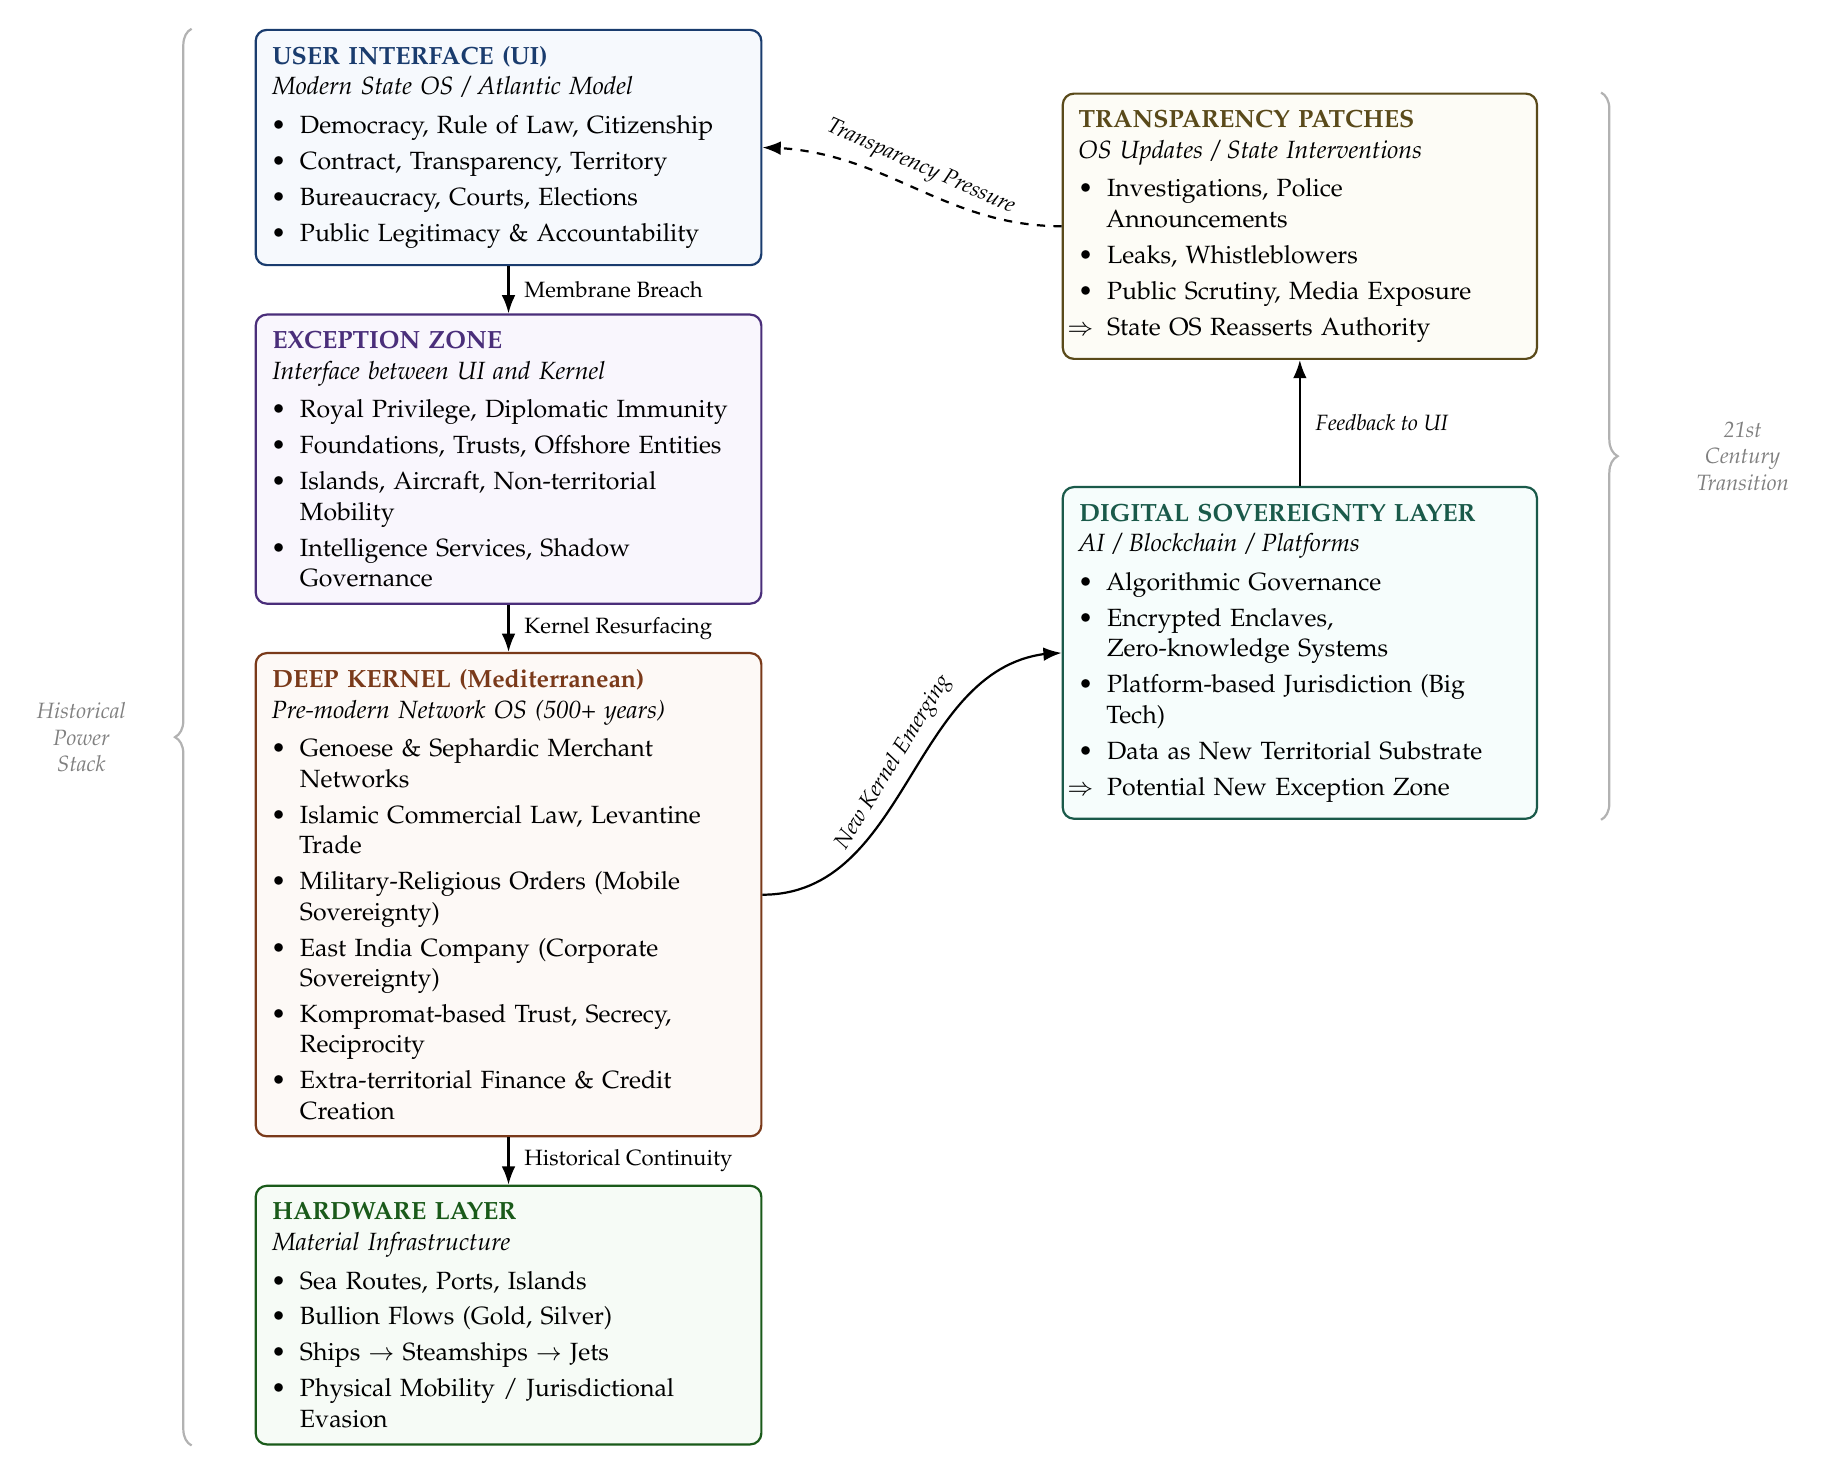
\begin{tikzpicture}[
  font=\small,
  node distance=6mm,
  box/.style={
    draw,
    rounded corners,
    thick,
    align=left,
    inner sep=6pt,
    text width=60mm,
  },
  boxR/.style={
    draw,
    rounded corners,
    thick,
    align=left,
    inner sep=6pt,
    text width=56mm,
  },
  arrow/.style={-Latex, thick},
  darrow/.style={-Latex, thick, dashed},
]

% -------------------------------------------------------
% LEFT STACK (Historical Power)
% -------------------------------------------------------

\node[box, fill=lightblue!60, draw=uiblue] (ui) {%
  \textbf{\textcolor{uiblue}{USER INTERFACE (UI)}}\\
  \textit{\small Modern State OS / Atlantic Model}\\[3pt]
  \begin{itemize}[leftmargin=10pt, itemsep=0pt, topsep=0pt]
    \item Democracy, Rule of Law, Citizenship
    \item Contract, Transparency, Territory
    \item Bureaucracy, Courts, Elections
    \item Public Legitimacy \& Accountability
  \end{itemize}
};

\node[box, fill=lightpurple!60, draw=ezpurple, below=of ui] (ez) {%
  \textbf{\textcolor{ezpurple}{EXCEPTION ZONE}}\\
  \textit{\small Interface between UI and Kernel}\\[3pt]
  \begin{itemize}[leftmargin=10pt, itemsep=0pt, topsep=0pt]
    \item Royal Privilege, Diplomatic Immunity
    \item Foundations, Trusts, Offshore Entities
    \item Islands, Aircraft, Non-territorial Mobility
    \item Intelligence Services, Shadow Governance
  \end{itemize}
};

\node[box, fill=lightorange!60, draw=kernelbrown, below=of ez] (kernel) {%
  \textbf{\textcolor{kernelbrown}{DEEP KERNEL (Mediterranean)}}\\
  \textit{\small Pre-modern Network OS (500+ years)}\\[3pt]
  \begin{itemize}[leftmargin=10pt, itemsep=0pt, topsep=0pt]
    \item Genoese \& Sephardic Merchant Networks
    \item Islamic Commercial Law, Levantine Trade
    \item Military-Religious Orders (Mobile Sovereignty)
    \item East India Company (Corporate Sovereignty)
    \item Kompromat-based Trust, Secrecy, Reciprocity
    \item Extra-territorial Finance \& Credit Creation
  \end{itemize}
};

\node[box, fill=lightgreen!60, draw=hwgreen, below=of kernel] (hw) {%
  \textbf{\textcolor{hwgreen}{HARDWARE LAYER}}\\
  \textit{\small Material Infrastructure}\\[3pt]
  \begin{itemize}[leftmargin=10pt, itemsep=0pt, topsep=0pt]
    \item Sea Routes, Ports, Islands
    \item Bullion Flows (Gold, Silver)
    \item Ships $\rightarrow$ Steamships $\rightarrow$ Jets
    \item Physical Mobility / Jurisdictional Evasion
  \end{itemize}
};

% -------------------------------------------------------
% RIGHT STACK (21st Century)
% -------------------------------------------------------

\node[boxR, fill=lightyellow!60, draw=patchgold,
      right=38mm of ui, yshift=-10mm] (patch) {%
  \textbf{\textcolor{patchgold}{TRANSPARENCY PATCHES}}\\
  \textit{\small OS Updates / State Interventions}\\[3pt]
  \begin{itemize}[leftmargin=10pt, itemsep=0pt, topsep=0pt]
    \item Investigations, Police Announcements
    \item Leaks, Whistleblowers
    \item Public Scrutiny, Media Exposure
    \item[$\Rightarrow$] State OS Reasserts Authority
  \end{itemize}
};

\node[boxR, fill=lightteal!60, draw=digitalteal,
      below=16mm of patch] (digital) {%
  \textbf{\textcolor{digitalteal}{DIGITAL SOVEREIGNTY LAYER}}\\
  \textit{\small AI / Blockchain / Platforms}\\[3pt]
  \begin{itemize}[leftmargin=10pt, itemsep=0pt, topsep=0pt]
    \item Algorithmic Governance
    \item Encrypted Enclaves, Zero-knowledge Systems
    \item Platform-based Jurisdiction (Big Tech)
    \item Data as New Territorial Substrate
    \item[$\Rightarrow$] Potential New Exception Zone
  \end{itemize}
};

% -------------------------------------------------------
% ARROWS: Left stack (vertical)
% -------------------------------------------------------

\draw[arrow] (ui.south) -- node[right=2pt]{\footnotesize Membrane Breach} (ez.north);
\draw[arrow] (ez.south) -- node[right=2pt]{\footnotesize Kernel Resurfacing} (kernel.north);
\draw[arrow] (kernel.south) -- node[right=2pt]{\footnotesize Historical Continuity} (hw.north);

% -------------------------------------------------------
% ARROWS: Cross connections
% -------------------------------------------------------

% Deep Kernel → Digital (horizontal)
\draw[arrow] (kernel.east) to[out=0, in=180]
  node[above, sloped, font=\footnotesize]{\textit{New Kernel Emerging}}
  (digital.west);

% Digital → Transparency Patch (upward)
\draw[arrow] (digital.north) -- node[right=2pt, font=\footnotesize]{\textit{Feedback to UI}} (patch.south);

% Transparency Patch → UI (dashed, curved)
\draw[darrow] (patch.west) to[out=180, in=0]
  node[above, sloped, font=\footnotesize]{\textit{Transparency Pressure}}
  (ui.east);

% -------------------------------------------------------
% BRACES
% -------------------------------------------------------

\draw[decorate, decoration={brace, amplitude=6pt, mirror}, thick, color=gray!60]
  ([xshift=-8mm] ui.north west) --
  ([xshift=-8mm] hw.south west)
  node[midway, xshift=-14mm, align=center, font=\footnotesize\itshape, color=gray]{Historical\\Power\\Stack};

\draw[decorate, decoration={brace, amplitude=6pt}, thick, color=gray!60]
  ([xshift=8mm] patch.north east) --
  ([xshift=8mm] digital.south east)
  node[midway, xshift=18mm, align=center, font=\footnotesize\itshape, color=gray]{21st\\Century\\Transition};

\end{tikzpicture}
}% end resizebox

\end{figure}

% ============================================================
\section{The Atlantic Revolutions: Installing the Modern State OS}
% ============================================================

\subsection{Fiscal Collapse as a Structural Trigger}

The American Revolution (1776) and the French Revolution (1789) constituted
a profound restructuring of political legitimacy in the Atlantic world.
France's intervention in the American War of Independence precipitated fiscal
collapse, forcing the termination of \emph{ancien r\'egime} governance
structures.

In 1781, Jacques Necker published the \emph{Compte rendu au Roi}, the first
public disclosure of royal finances in French history. This unprecedented act
of transparency exposed the opacity of monarchical governance and functioned
as an early institutional update toward public accountability --- a
transparency patch applied to an aging system.

\subsection{Contract, Legality, and Transparency}

The Atlantic Revolutions replaced legitimacy grounded in divine sanction,
hereditary privilege, and corporate estates with governance grounded in
contract, legality, and transparency. In the United States, Protestant moral
frameworks supported a durable regime of negative liberty. In France, the
elevation of Reason as a sovereign principle fostered positive liberty,
culminating in the Terror.

In both cases, revolutionary transformation did not eliminate older
extra-territorial networks of power. These persisted as a parallel structural
logic beneath the modern state OS --- not as remnants to be overcome, but as
constitutive counterweights to territorial sovereignty.

% ============================================================
\section{The Genealogy of Exception: Deep Kernels Beyond the State OS}
% ============================================================

The modern state aspires to align law with territory. Yet historically, zones
of exception --- spaces where law is suspended, negotiated, or selectively
applied --- have persisted as sites of operational power. These zones do not
simply predate the state; they co-exist with it, sometimes in tension,
sometimes in symbiosis.

\subsection{Military-Religious Orders: Mobile Sovereignty}

Orders such as the Knights Templar and the Knights of Malta exercised
taxation privileges, military autonomy, and diplomatic independence across
territorial borders. They represent early structural instances of
\textbf{mobile sovereignty}: forms of authority operating beyond any single
jurisdiction while interacting continuously with territorial powers.

\subsection{Chartered Companies: Corporate Sovereignty}

The East India Company exercised authority typically associated with states
--- warfare, taxation, currency issuance, territorial governance --- while
remaining formally a commercial entity. It functioned as a quasi-sovereign
kernel operating parallel to formal state authority, instantiating the
structural logic of network power within a corporate form.

\subsection{Tax Havens: Encrypted Zones of Modern Governance}

In the twentieth century, offshore financial jurisdictions emerged as
encrypted spaces circumventing state taxation, regulatory oversight, and
financial transparency. Structurally, these spaces recapitulate the logic of
earlier exception zones: partial insulation from territorial law, serving
concentrated interests through jurisdictional arbitrage.

Across these cases, no single continuous organization is asserted. Rather, a
recurring pattern emerges: a non-territorial structural logic through which
power operates alongside formal sovereignty.

% ============================================================
\section{The Epstein Affair: Structural Visibility of the Deep Kernel}
% ============================================================

\subsection{An Instance of Structural Visibility, Not Proof of a Theory}

Interpreting the Epstein affair solely as a criminal scandal obscures its
analytical utility. The episode is treated here not as evidence that the
theoretical model is correct, but as a \textbf{moment of structural
visibility}: an instance in which network-based power relations, ordinarily
opaque, became publicly legible through legal and journalistic scrutiny.

The affair illuminates the interface between two co-existing operational
logics: the modern state OS, governed by contract and transparency; and a
network logic, governed by encrypted social ties, mutual exposure, and
jurisdictional mobility. It stress-tests the model by revealing the friction
between these layers when state institutions attempt to access domains
ordinarily insulated from legal scrutiny.

\subsection{Two Operating Logics in Tension}

\begin{table}[H]
\centering
\caption{Structural Comparison: Modern State OS vs.\ Network Power}
\label{tab:comparison}
\vspace{4pt}
\renewcommand{\arraystretch}{1.4}
\begin{tabularx}{\textwidth}{>{\bfseries}p{3.2cm} X X}
\toprule
Dimension &
\textbf{Modern State OS} \newline {\small\itshape Atlantic Model} &
\textbf{Network Power} \newline {\small\itshape Mediterranean Model} \\
\midrule
Basis of Trust &
Contract, judiciary, transparency &
Reciprocity, silence, mutual exposure \\
Spatial Logic &
Fixed territory &
Islands, aircraft, foundations --- jurisdictional diffusion \\
Primary Actors &
Citizens, bureaucracies &
Foundations, intelligence networks, kinship alliances \\
Legitimacy Source &
Public consent, legal procedure &
Encrypted social ties, network loyalty \\
\bottomrule
\end{tabularx}
\end{table}

The island operated as a jurisdictionally insulated enclave; private aircraft
enabled mobility across legal regimes. The binding mechanism was not
contractual legality but encrypted social ties grounded in mutual exposure.
Whether this pattern is unique to this case or structurally representative is
a question the model raises rather than definitively answers.

% ============================================================
\section{Hegemonic Transition: AI and the Rise of Digital Sovereignty}
% ============================================================

\subsection{Transparency vs.\ Neo-Feudal Encryption}

The twenty-first century is witnessing a shift from territorial sovereignty
toward digitally mediated authority. Artificial intelligence and distributed
ledger technologies may function either as instruments of radical transparency
or as infrastructures enabling digitally fortified exception zones beyond
public oversight.

This dual potential reflects a fundamental normative ambiguity embedded in
digital infrastructures --- one that mirrors the structural ambiguity observed
in earlier exception zones. The question is not whether such zones will
emerge, but under what conditions they become sites of accountability or sites
of opacity.

\subsection{AI as an Emerging Exception Zone}

AI systems may constitute new domains of quasi-sovereign authority, executing
decision processes beyond conventional legal frameworks. The structural analogy
with earlier forms of mobile sovereignty --- military orders, chartered
companies --- is not causal but formal: it identifies a recurring logic in
which technically complex, operationally opaque systems interact with
territorial governance in asymmetric ways.

Following Arrighi's analysis of systemic cycles \cite{arrighi1994}, the
current hegemonic transition toward multipolarity may accelerate the
proliferation of such exception zones, as states and networks compete to
define the terms of digital sovereignty.

% ============================================================
\section{Transparency Events as OS-Level Interventions}
% ============================================================

Periodically, state institutions attempt to access domains traditionally
insulated from legal scrutiny. These moments --- \textbf{transparency events}
--- represent OS-level interventions: instances in which the visible
governance layer reasserts authority over the network layer.

Such moments belong to a longer historical lineage: parliamentary challenges
to royal prerogative in the seventeenth century; fiscal transparency reforms
in the late eighteenth century; contemporary legal proceedings involving
transnational networks. In each case, the state OS attempts to render legible
what has operated beneath or alongside it.

Recent examples across multiple jurisdictions --- law enforcement actions
targeting offshore financial structures, legal proceedings involving
intelligence-adjacent networks, regulatory interventions into AI governance
--- illustrate this recurring dynamic. The outcome of such interventions is
not predetermined: they may produce genuine transparency, surface-level
accountability while leaving deeper structures intact, or trigger adaptation
in the network layer.

These events are significant not because they definitively resolve the tension
between the two layers, but because they mark the sites where that tension
becomes visible and contestable.

% ============================================================
\clearpage
\section*{Conclusion: Recovering Administrative Insight into Historical Infrastructure}
% ============================================================

This study has argued that the modern state constitutes the visible interface
of governance, while a recurring structural logic --- network-based,
non-territorial, operating through exception and encrypted social ties ---
persists alongside it. This is a \textbf{model for understanding}, not a
proof of conspiracy.

The Epstein affair provided one instance where the boundary between these
layers became publicly visible. AI governance is emerging as a new site where
the same structural tension will be played out.

As artificial intelligence reshapes governance architectures, the central
question is whether emerging systems will prioritize transparency, encryption,
or hybrid forms combining both. Understanding sovereignty as a layered
architecture --- following Braudel's \emph{longue dur\'ee}, Schmitt's theory
of exception, and Arrighi's hegemonic cycles --- is essential for evaluating
the future of governance, accountability, and digital authority.

\begin{bquote}
Recovering analytical insight into the deep infrastructures of history is not
merely an academic task. It is a prerequisite for navigating the political
transformations of the twenty-first century with clear eyes.
\end{bquote}

\vspace{16pt}
\begin{center}
  \textcolor{rulecolor}{\rule{0.6\textwidth}{0.4pt}}
\end{center}

% ============================================================
% References
% ============================================================
\clearpage
\begin{thebibliography}{9}

\bibitem{arrighi1994}
Arrighi, G. (1994).
\textit{The Long Twentieth Century: Money, Power, and the Origins of Our Times}.
Verso.

\bibitem{braudel1949}
Braudel, F. (1949).
\textit{La M\'editerran\'ee et le monde m\'editerran\'een \`a l'\'epoque de Philippe II}.
Armand Colin.

\bibitem{braudel1979}
Braudel, F. (1979).
\textit{Civilisation mat\'erielle, \'economie et capitalisme, XV\textsuperscript{e}--XVIII\textsuperscript{e} si\`ecle}.
Armand Colin.

\bibitem{schmitt1922}
Schmitt, C. (1922).
\textit{Politische Theologie}.
Duncker \& Humblot.
[English trans.: \textit{Political Theology}, trans.\ G.\ Schwab, MIT Press, 1985.]

\bibitem{wallerstein1974}
Wallerstein, I. (1974--2011).
\textit{The Modern World-System} (4 vols.).
Academic Press / University of California Press.

\end{thebibliography}

\vspace{12pt}
\noindent\small\textcolor{blockquotegray}{%
\textbf{Version Notes --- v1.1:}
(1)~Methodological Preface clarifying the paper's status as a theoretical model;
(2)~Refined definition of the Mediterranean deep kernel as structural logic;
(3)~Repositioning of the Epstein affair as an instance of structural visibility;
(4)~Explicit theoretical dialogue with Braudel, Arrighi, and Schmitt;
(5)~Abstraction of Chapter~5 to emphasize recurring institutional patterns.
TikZ diagram integrated as Figure~\ref{fig:diagram}.}

\end{document}
